\documentclass[]{scrartcl}
\usepackage{lmodern}
\usepackage{amssymb,amsmath}
\usepackage{ifxetex,ifluatex}
\usepackage{fixltx2e} % provides \textsubscript
\ifnum 0\ifxetex 1\fi\ifluatex 1\fi=0 % if pdftex
  \usepackage[T1]{fontenc}
  \usepackage[utf8]{inputenc}
\else % if luatex or xelatex
  \ifxetex
    \usepackage{mathspec}
  \else
    \usepackage{fontspec}
  \fi
  \defaultfontfeatures{Ligatures=TeX,Scale=MatchLowercase}
\fi
% use upquote if available, for straight quotes in verbatim environments
\IfFileExists{upquote.sty}{\usepackage{upquote}}{}
% use microtype if available
\IfFileExists{microtype.sty}{%
\usepackage{microtype}
\UseMicrotypeSet[protrusion]{basicmath} % disable protrusion for tt fonts
}{}
\usepackage{hyperref}
\hypersetup{unicode=true,
            pdftitle={Angabe},
            pdfauthor={Team\ldots{}},
            pdfborder={0 0 0},
            breaklinks=true}
\urlstyle{same}  % don't use monospace font for urls
\IfFileExists{parskip.sty}{%
\usepackage{parskip}
}{% else
\setlength{\parindent}{0pt}
\setlength{\parskip}{6pt plus 2pt minus 1pt}
}
\setlength{\emergencystretch}{3em}  % prevent overfull lines
\providecommand{\tightlist}{%
  \setlength{\itemsep}{0pt}\setlength{\parskip}{0pt}}
\setcounter{secnumdepth}{5}
% Redefines (sub)paragraphs to behave more like sections
\ifx\paragraph\undefined\else
\let\oldparagraph\paragraph
\renewcommand{\paragraph}[1]{\oldparagraph{#1}\mbox{}}
\fi
\ifx\subparagraph\undefined\else
\let\oldsubparagraph\subparagraph
\renewcommand{\subparagraph}[1]{\oldsubparagraph{#1}\mbox{}}
\fi

\usepackage{graphicx}
\usepackage{array}
\usepackage{ragged2e}
\usepackage[section]{placeins}
\makeatletter
\AtBeginDocument{%
  \expandafter\renewcommand\expandafter\subsection\expandafter{%
    \expandafter\@fb@secFB\subsection
  }%
}
\makeatother

\title{Modell eines Insel-Callshops}
\providecommand{\subtitle}[1]{}
\subtitle{2. Projekt zu Modellierung und Simulation}
\author{Daniel Graf, Dimitrie Diez, Arne Schöntag, Peter Müller}
\date{}

\begin{document}

\maketitle

\tableofcontents

\section{Einführung}
Simulationen haben in der moderne einen sehr hohen Stellenwert erlangt, da durch sie zahlreiche, oftmals sehr genaue, Zukunftsprognosen erstellt werden können. Das Thema dieser Studienarbeit ist die Simulation eines Callshops, bzw. des Telefons in einem Callshop, in einem Inseldorf. Dieser wird für günstige Telefonate ins Ausland verwendet. 

Mit Hilfe der Simulation sollen anschließend Aussagen bezüglich der zukünftigen Auslastung des Telefons getroffen werden können. Konkret wird die Fragestellung betrachtet, ob ein zweites Telefon im Callshop sinnvoll oder unnötig ist. 

Als Basis für die erläuterten Prognosen werden folgende Werte der Simulation ermittelt:
\begin{itemize}
	\item mittlere Länge der Warteschlage (anstehende Kunden)
	\item mittlere Wartezeit bis zum Telefonat
	\item mittlere Verweildauer im Callshop (Wartezeit + Gesprächsdauer) 
	\item Mittlere Auslastung des Telefons
\end{itemize}

\section{Beschreibung des Modells}
Für die Simulation des Insel-Callshops wird ein Warteschlagenmodell mit jeweils einem Client und Server verwendet. Jede Person die den CallShop betritt wird durch einen neuen Client repräsentiert. Das Telefon des Shops ist durch den Server dargestellt. Möchte eine Person das Telefon zu einem Zeitpunkt benützen, zu dem bereits eine andere Person telefoniert, muss sie sich hinten anstellen und warten, bis die Person ihr Telefonat beendet hat. Im Modell wird dieses durch eine Warteschlage (Queue) realisiert, in die sich die wartenden Clients einordnen und nach dem FIFO (first in first out) Prinzip bedient werden. 

Im Modell werden sowohl die Ankunftszeiten der Clients, als auch die Dauer der Telefonate durch eine negative Exponentialverteilung beschrieben, da diese sehr nah an den real beoachteten Verhalten liegt. Der mathematische Hintergrund liegt in der Eigenschaft der Exponentialfunktion zugrunde. Die Exponentialverteilung ist die einzige kontinuierliche Verteilung, welche zugleich die Markoveigenschaft, die sogenannte Gedächtnislosigkeit, erfüllt. Diese besagt, dass die seit dem letzten Ereignis vergangene Zeit (in diesem Beispiel Anrufer) keinen Einfluss auf die Verteilung der Zeit bis zum nächsten Ereignis (bis zum nächsten Anruf) hat. 
Quelle: http://www.mathepedia.de/Exponentialverteilung.aspx


\section{Anforderungen/Requirements}

\section{Softwaredesign}

Der Aufbau der Anwendung wurde im Team diskutiert und anschließend mittels UML spezifiziert.

Grundsätzlich wurde eine Ereignisorientierte Simulation (Discrete Event Simulation) mit einer Eventliste gewählt. Ursprünglich war geplant die Berechnung mit Mathematica auszuführen. Dies stellte sich aber als nicht performant und komplizierter als notwendig heraus. Alle geforderten Berechnungen wurden dann ebenfalls in das Java Programm eingeplant.

\subsection{Package time}

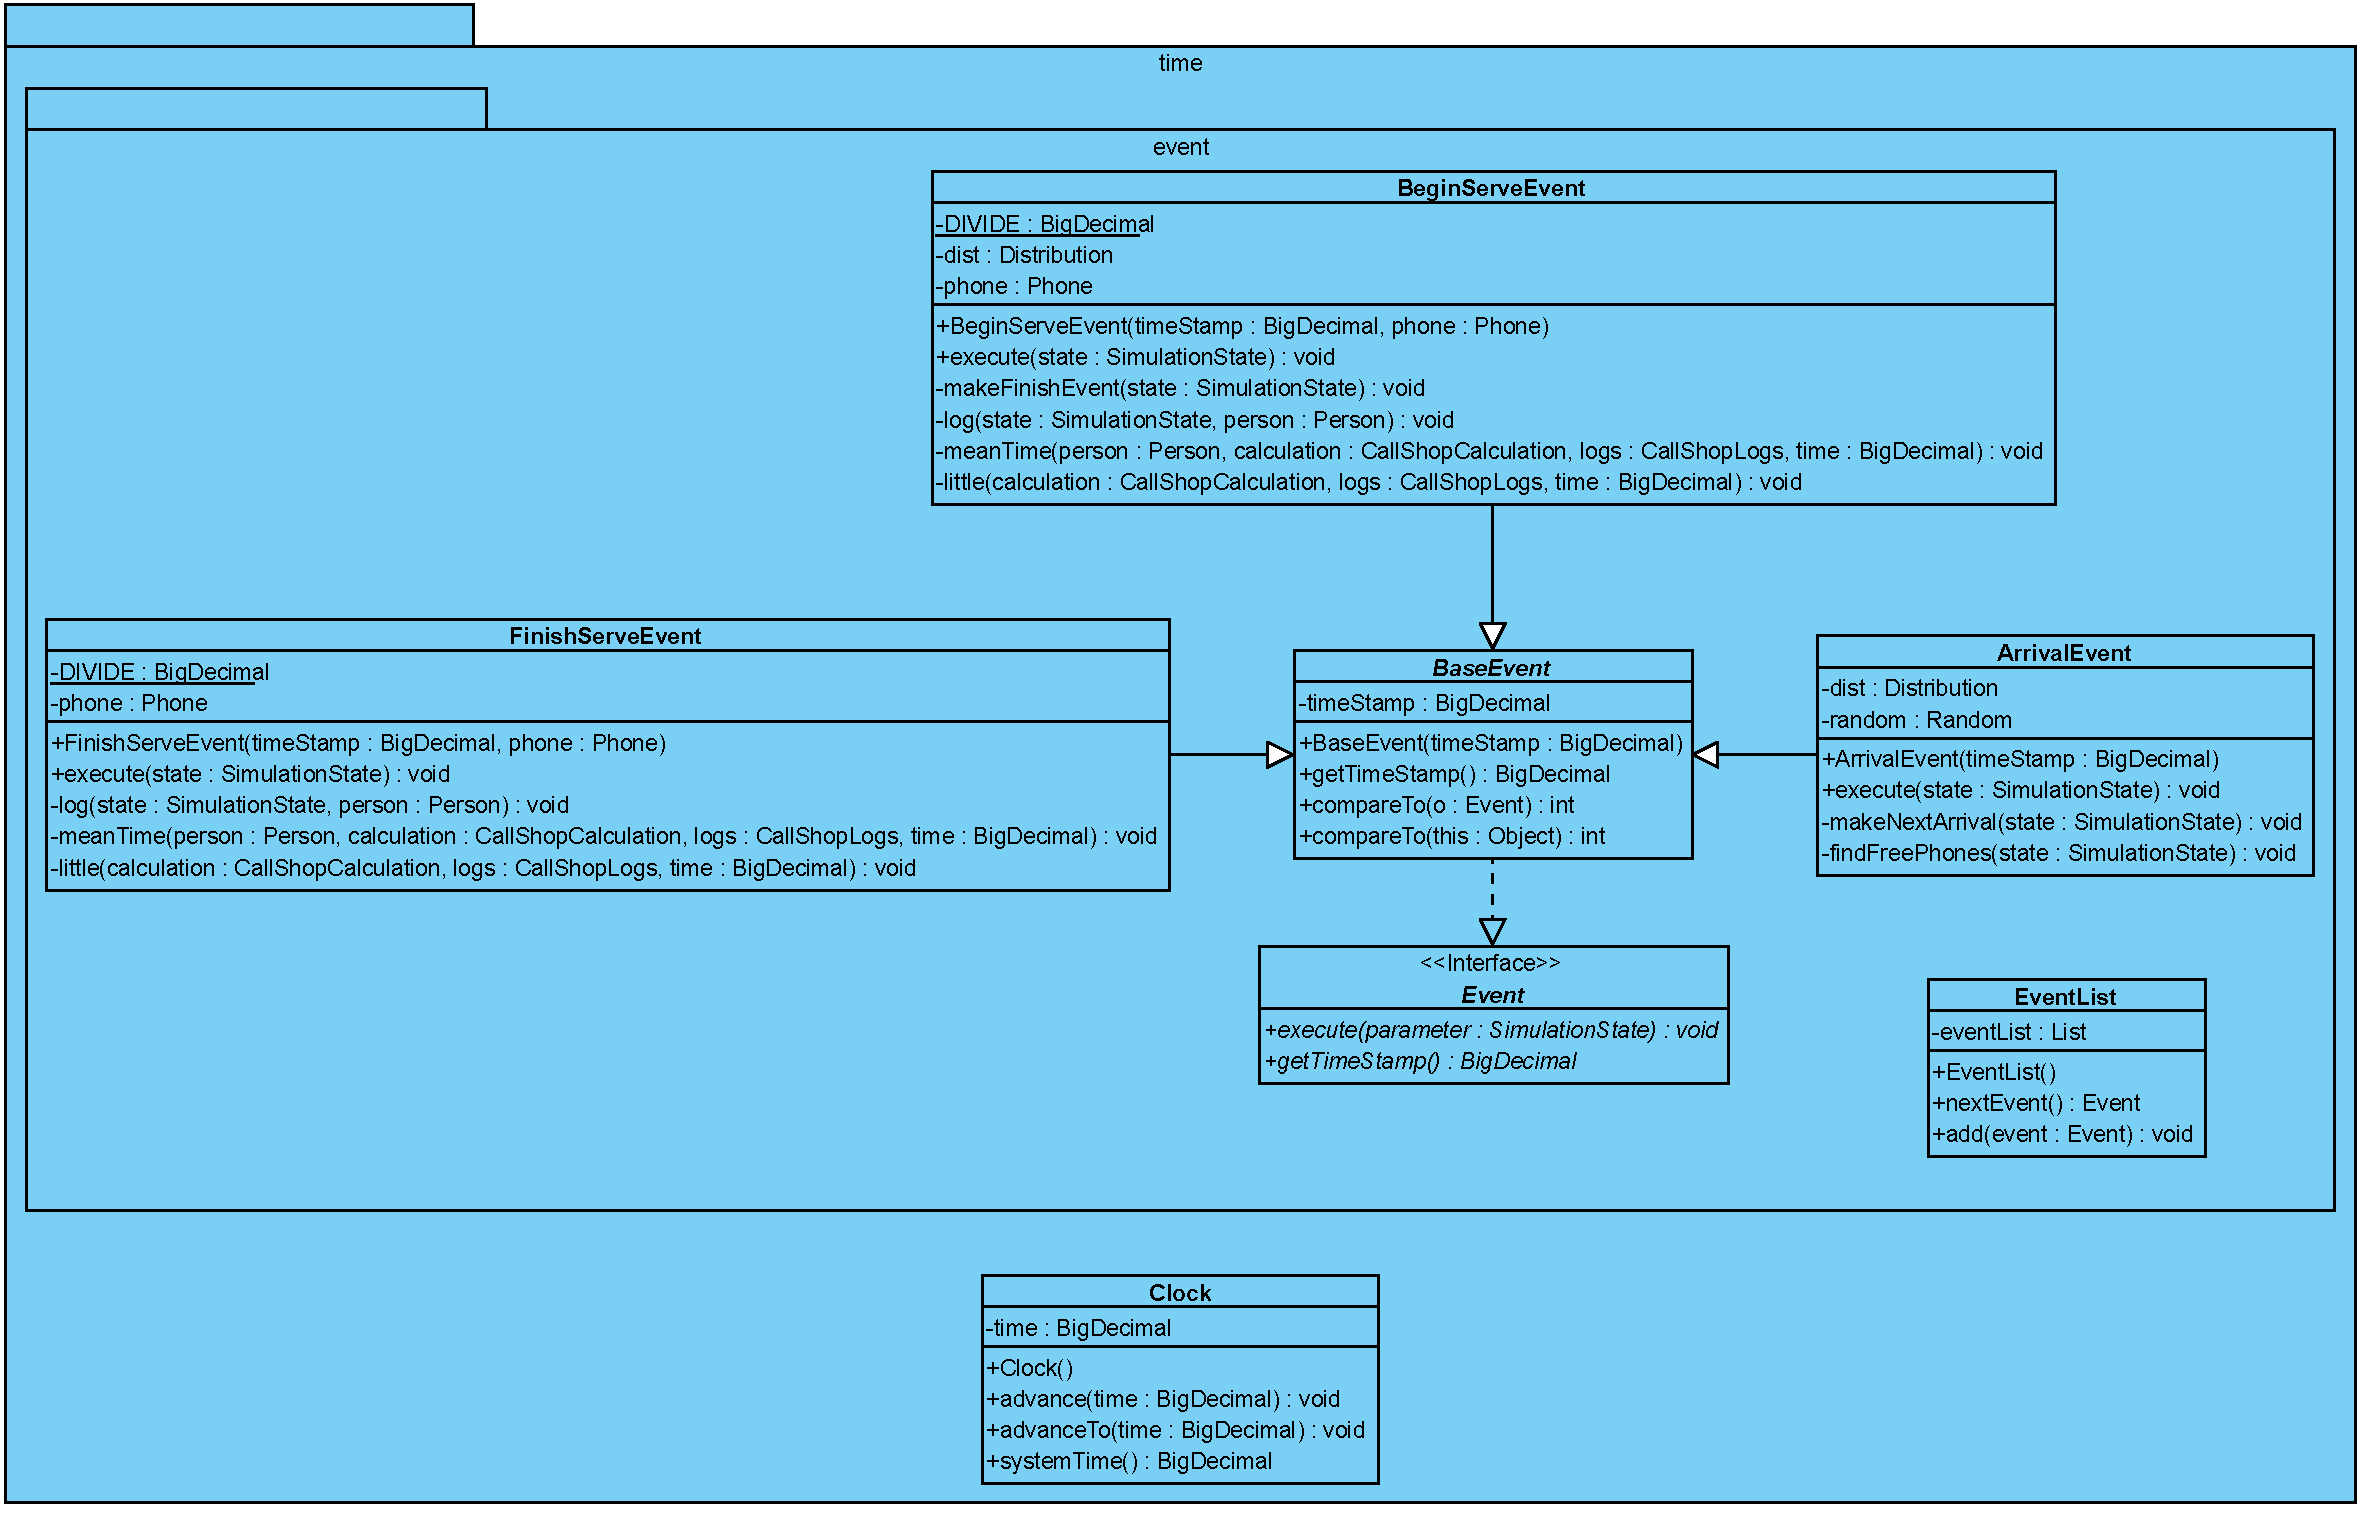
\includegraphics[scale=0.5]{abbildungen/uml/time.pdf}

In diesem Unterpaket finden sich alle notwendigen Klassen für die Ereignisorientierte Simulation. Die \texttt{Clock} hält die Simulationszeit und kann nur vorgestellt werden. 

Das Interface \texttt{Event} definiert ein Ereignis in der Simulation. Jedes Ereignis hat einen Zeitpunkt an dem es auftritt, sowie Logik, die zu diesem Zeitpunkt ausgeführt werden soll und potentiell den ganzen Zustand der Simulation verändern kann. Die \texttt{EventList} kann Ereignisse aufnehmen und immer das nächste Event mit den frühesten Zeitpunkt liefern. 

Die konkreten Events \texttt{Arrival, BeginServe, FinishServe} beschreiben die Ereignisse in der Callshop Problemstellung.

Abbildung \ref{fig:arrival-event} zeigt den Verlauf des Ereignisses für Arrival. Zunächst werden freie Telefone gesucht. Wird ein freies Telefon gefunden wird ein BeginServeEvent mit aktueller Zeit erstellt. Eine neue Person wird erstellt, ihre Ankunftszeit gespeichert, und die Person wird in die Schlange eingefügt. Zum Schluss wird das nächste ArrivalEvent erstellt, um fortlaufend neue Ankünfte zu haben.

Der Verlauf von BeginServe ist in Abbildung \ref{fig:beginserve-event} zu sehen. Die nächste (VIP oder normale) Person wird je nachdem, ob es sich um ein VIP Phone oder nicht handelt, aus der Liste geholt. Die Zeit vom Bearbeitungsbeginn wird für die Person gespeichert. Das FinishEvent wird direkt ermittelt und in die EventList eingetragen.

Das Ereignis FinishServe ist in Abbildung \ref{fig:finishserve-event} dargestellt. Die Person wird aus dem Phone entfernt. Ihre Endzeit wird gespeichert. Ist die Warteschlange nicht leer, wird direkt ein neues BeginServeEvent erstellt. 


\begin{figure}[ht]
	\centering
	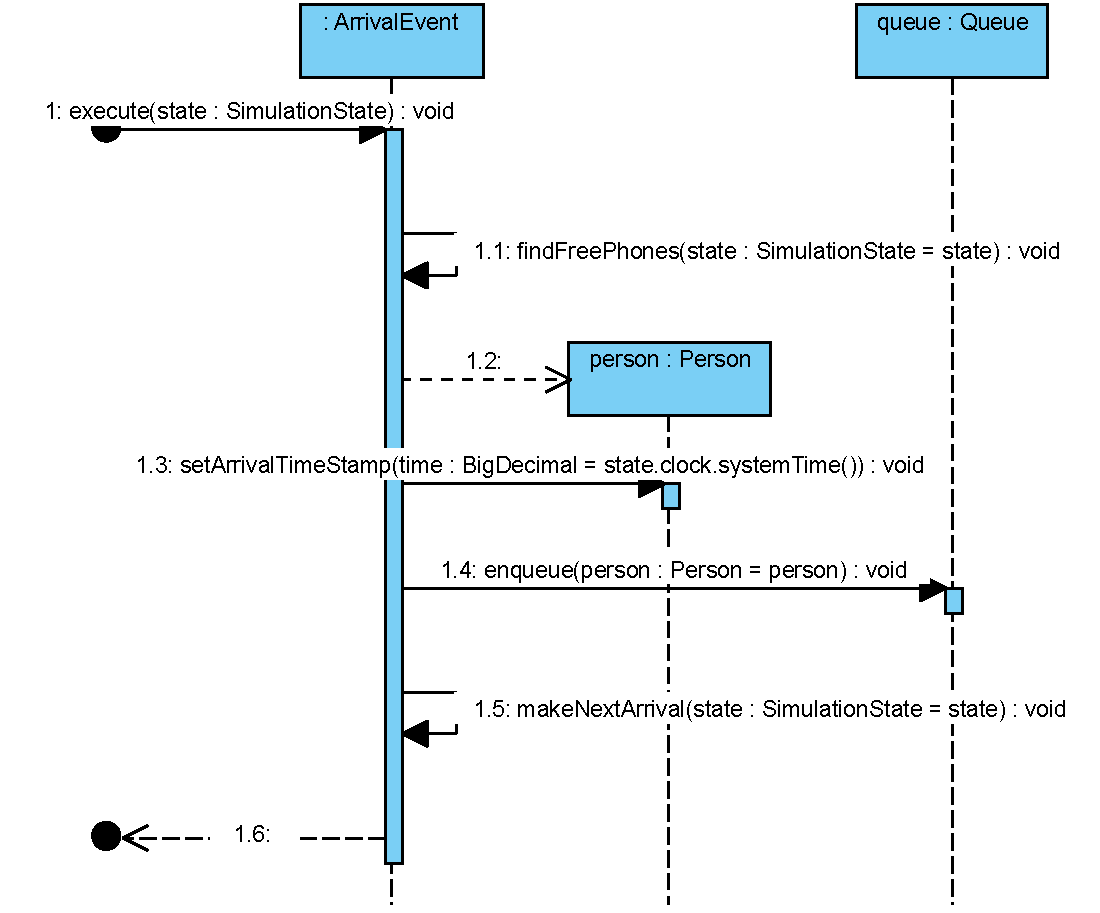
\includegraphics[scale=0.5]{abbildungen/uml/Arrival.pdf}
	\caption{Sequenzdiagramm für die Ausführung eines ArrivalEvent}
	\label{fig:arrival-event}
\end{figure}

\begin{figure}[ht]
	\centering
	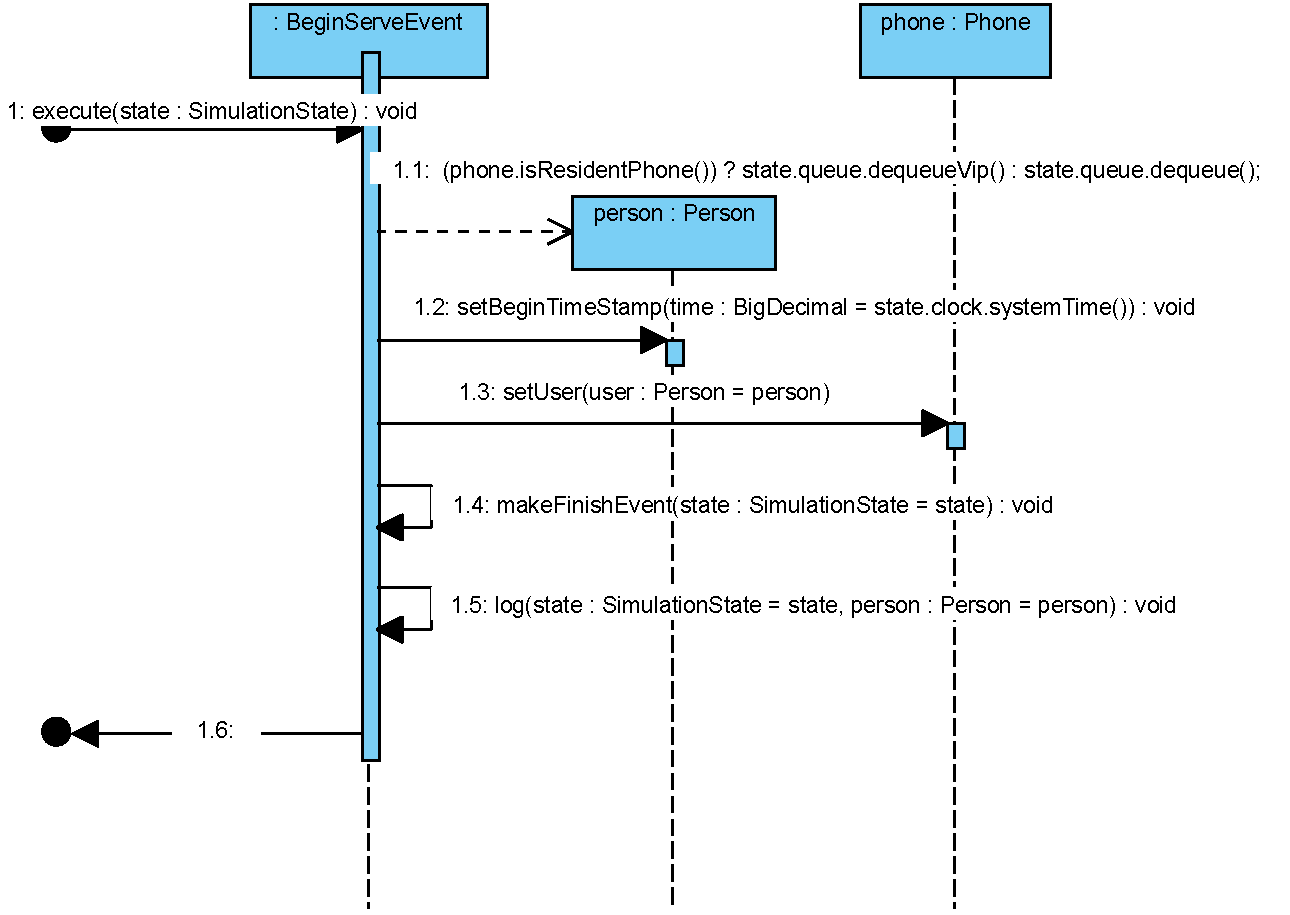
\includegraphics[scale=0.5]{abbildungen/uml/BeginServe.pdf}
	\caption{Sequenzdiagramm für die Ausführung eines BeginServeEvent}
	\label{fig:beginserve-event}
\end{figure}

\begin{figure}[ht]
	\centering
	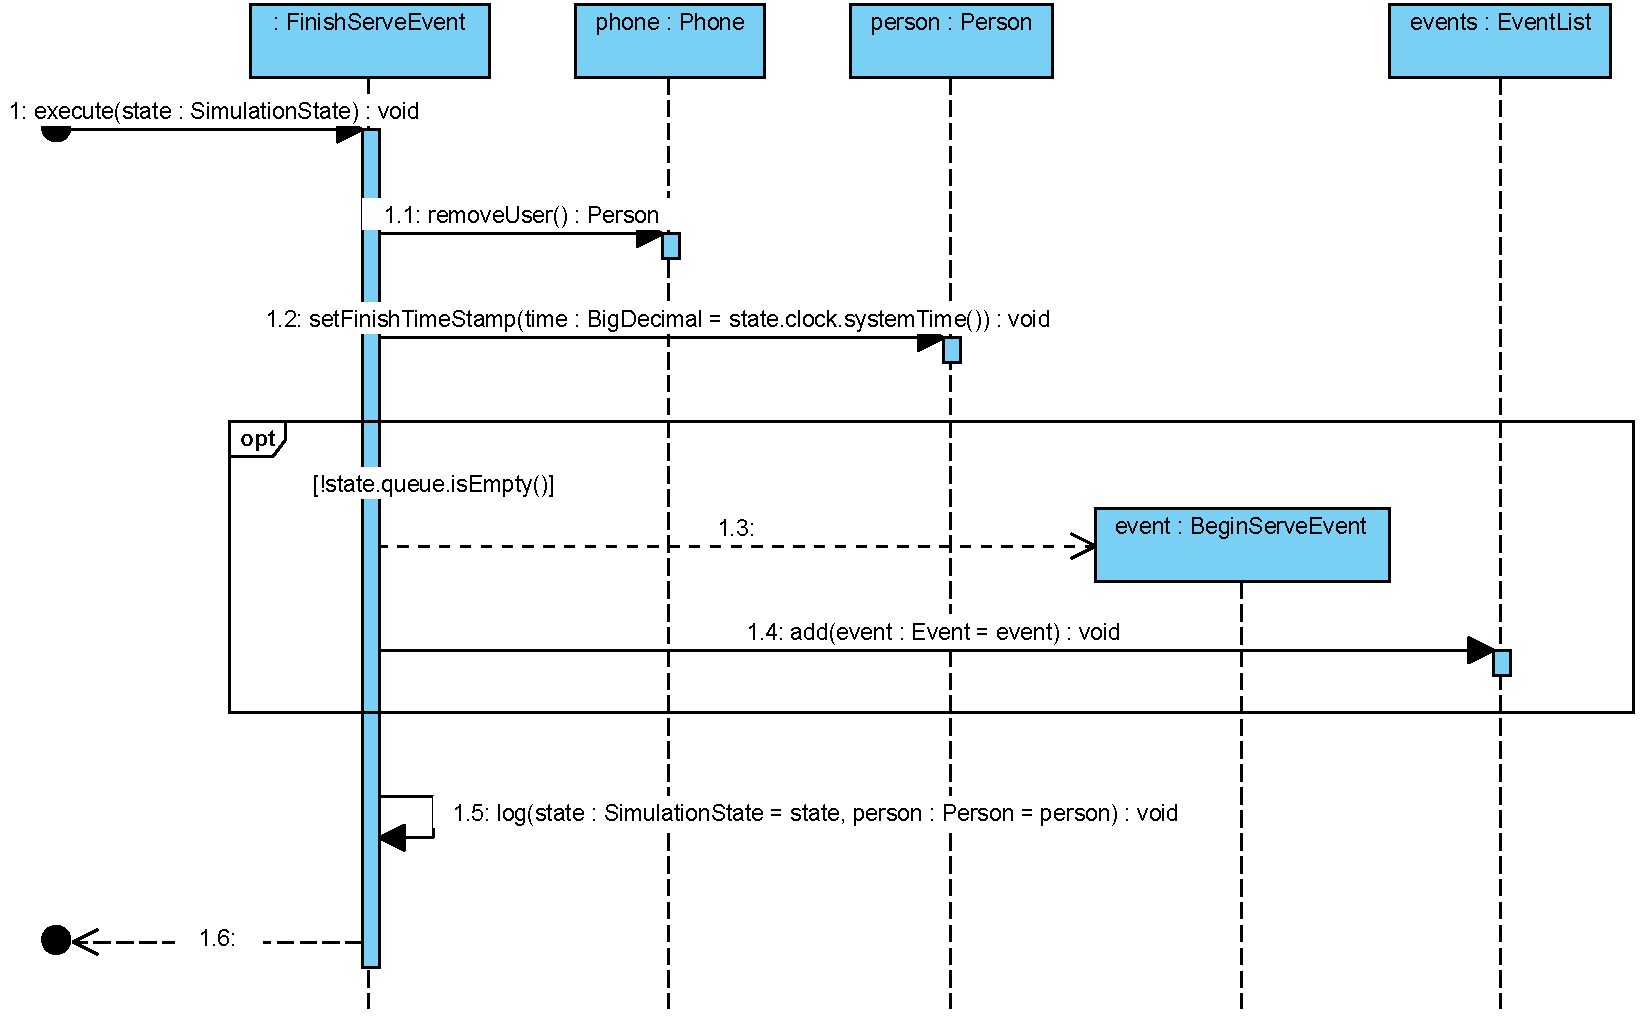
\includegraphics[scale=0.5]{abbildungen/uml/FinishServe.pdf}
	\caption{Sequenzdiagramm für die Ausführung eines FinishServeEvent}
	\label{fig:finishserve-event}
\end{figure}

\subsection{Package queue}

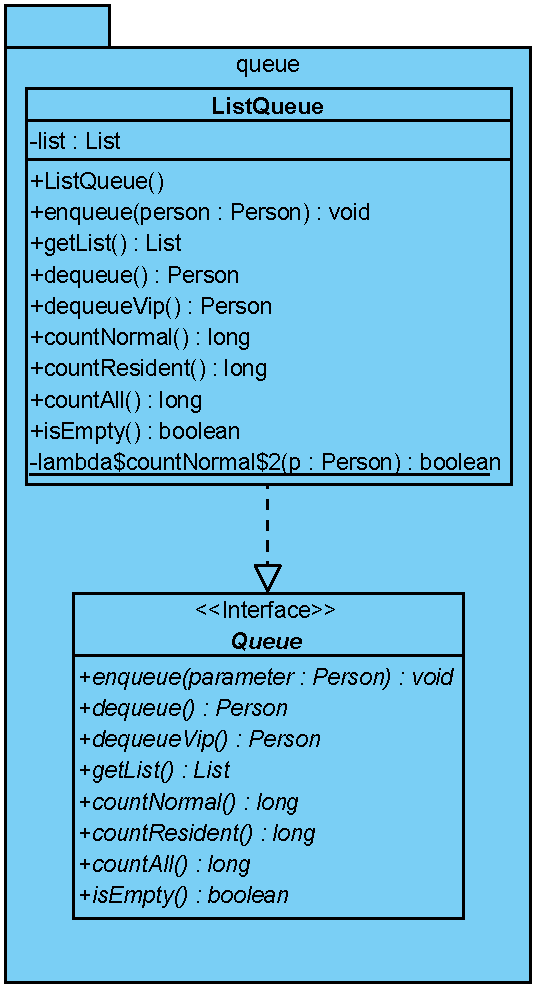
\includegraphics[scale=0.5]{abbildungen/uml/queue.pdf}

Die \texttt{Queue} ist eine FIFO-Warteschlange mit zugehörigen Operationen. Optional kann direkt auch der erste Resident (VIP) aus der Schlange entfernt werden. 

\subsection{Package distribution}

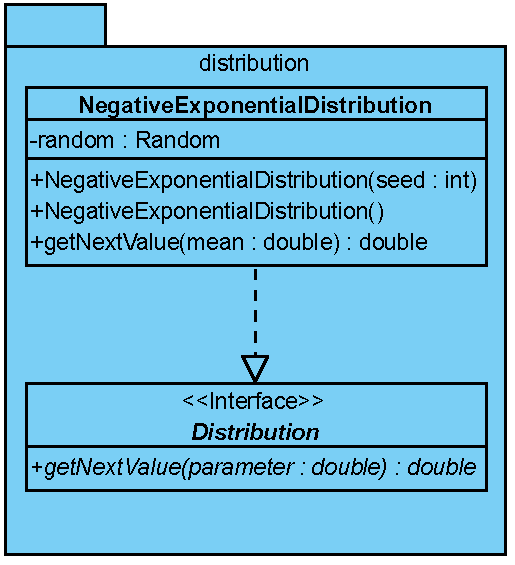
\includegraphics[scale=0.5]{abbildungen/uml/distribution.pdf}

Die Verteilung ist grundsätzlich eine negative Exponentialverteilung. Die 
Zufallszahlen können über einen Seed erstellt werden.

\subsection{Package domain}

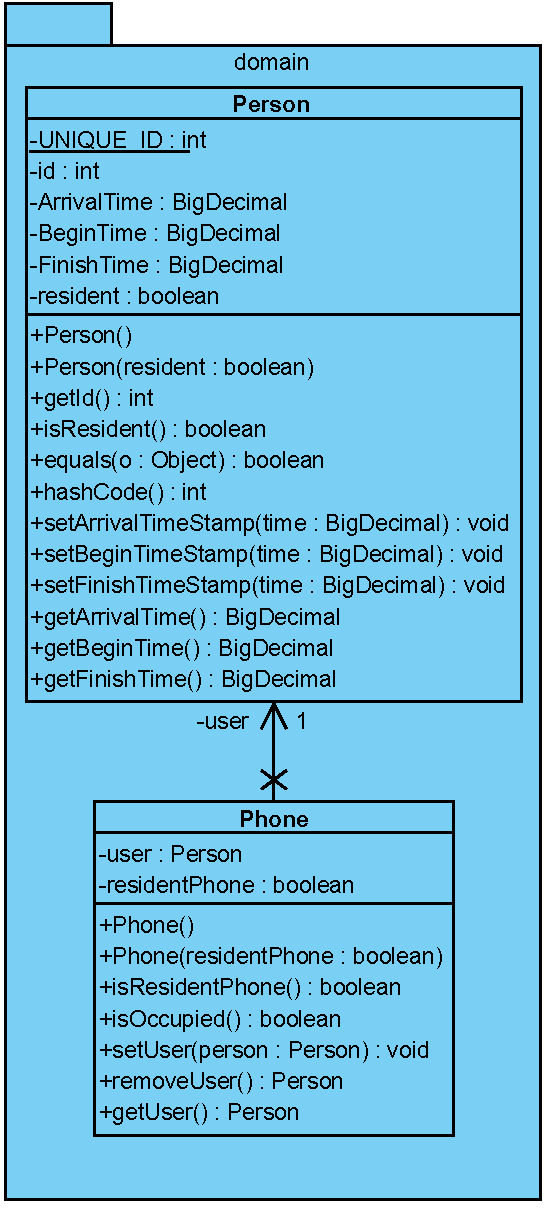
\includegraphics[scale=0.5]{abbildungen/uml/domain.pdf}


\texttt{domain} beschreibt alle notwendigen Datenstrukturen aus der Domäne des Callshops. Hier gibt es Personen und Telefone. Jede neue Person hat eine einzigartige ID und im Laufe der Simulation merkt sie sich ihre persönlichen Zeitpunkte.

Eine Person kann optional ein Resident (Vip) sein. Eine Telefon kann optional nur Residents (VIPs) annehmen.

\subsection{Package calculation, log}

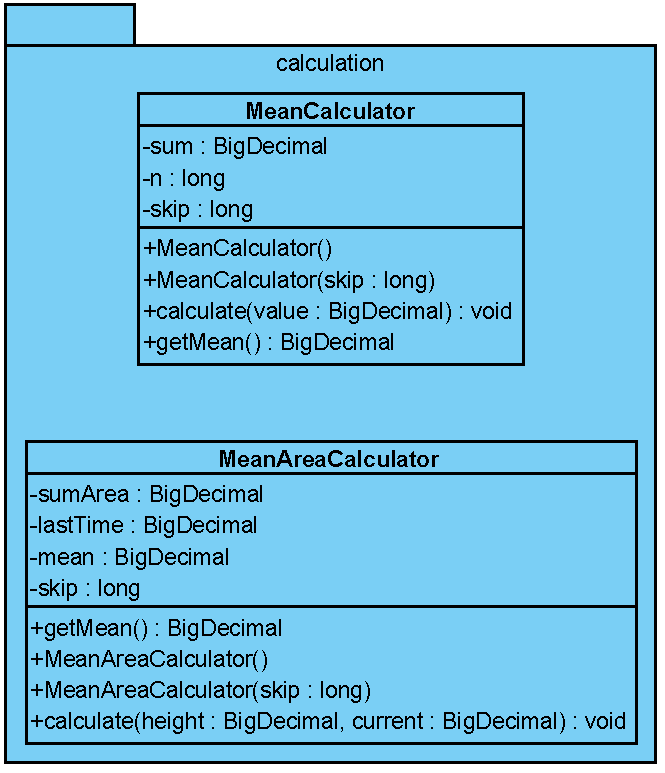
\includegraphics[scale=0.5]{abbildungen/uml/calculation.pdf}
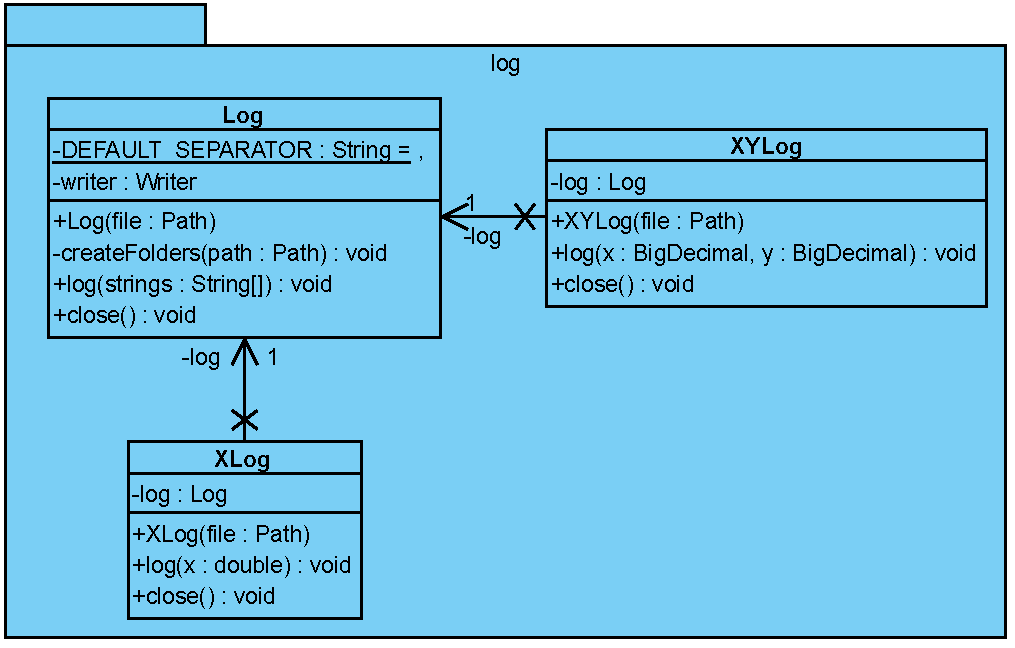
\includegraphics[scale=0.5]{abbildungen/uml/log.pdf}

Die allgemeine Berechnung für Mittelwerte ist in \texttt{calculation} gelöst.
Mit \texttt{log} können Ergebnisse in ein CSV Dokument gespeichert werden.

\subsection{Package config, modellbildung}

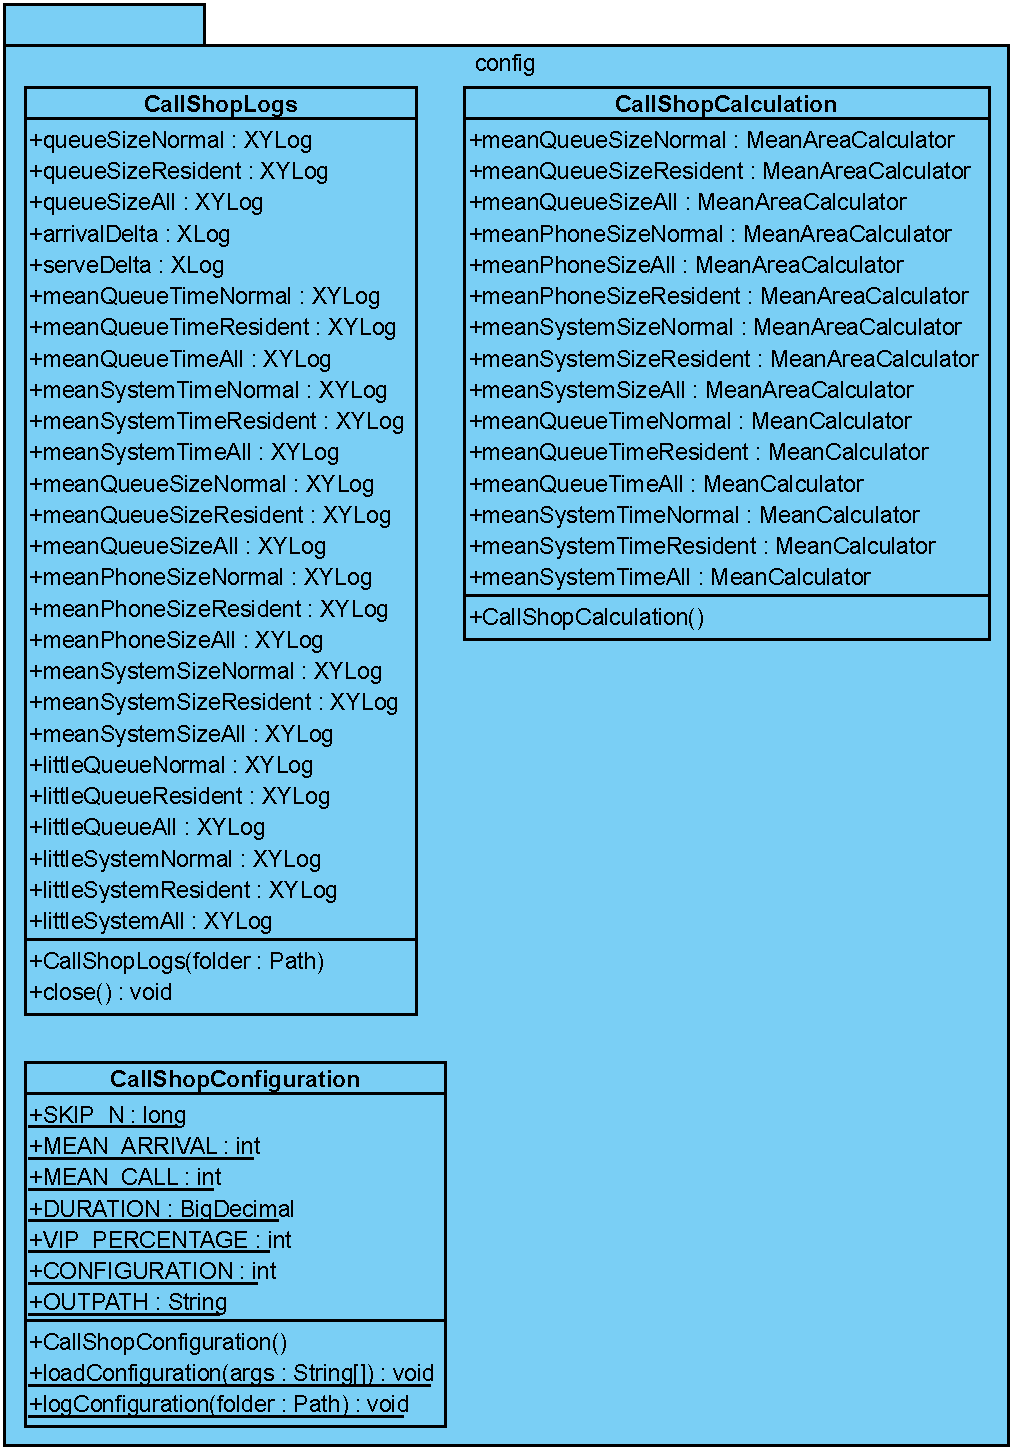
\includegraphics[scale=0.5]{abbildungen/uml/config.pdf}
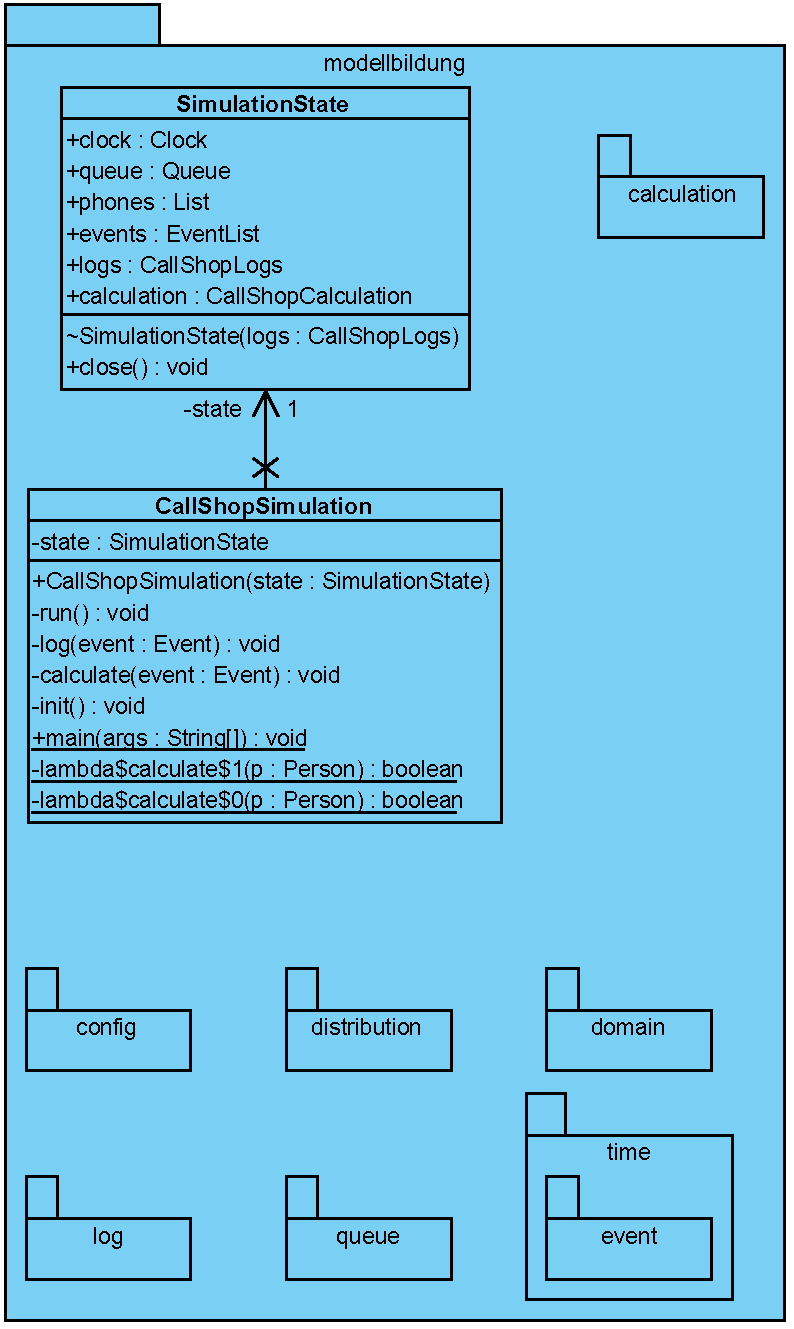
\includegraphics[scale=0.5]{abbildungen/uml/modellbildung.pdf}

In \texttt{config} ist die Konfiguration der Simulation zu finden. Die Logs und Mittelwert-Rechner für die aktuelle konkrete Simulation sind ebenfalls hier definiert.

Das Paket \texttt{modellbildung} beinhaltet alle zuvor beschriebenen Pakete und enthält die Simulationsklasse zum Starten sowie den groben Ablauf der Simulation. Der \texttt{SimulationState} hält den aktuellen Zustand der Simulation.

\section{Implementierung}

\section{Softwaretest}

\section{Simulation}

\section{Fazit}

\end{document}
